\section{Resultados y análisis}


\subsection{Verificación de la tensión}
En primer lugar se debe verificar que el ``convertidor de tensión'' en efecto pasa el rango de tensiones entre \SI{-24}{\volt} y \SI{24}{\volt} a un rango de tensión entre \SI{0}{\volt} y \SI{5}{\volt}. La figura \ref{volt-convert} muestra el resultado al pasar a la red resistiva una señal senoidal entre \SI{-24}{\volt} y \SI{24}{\volt}. Observe que en la salida la tensión en efecto está entre \SI{0}{\volt} y \SI{5}{\volt}. Por lo tanto, se concluye que la red resistiva está correctamente implementado, no hay riesgo de sobre-tensión que dañe el Arduino UNO.
\begin{figure}
    \centering
    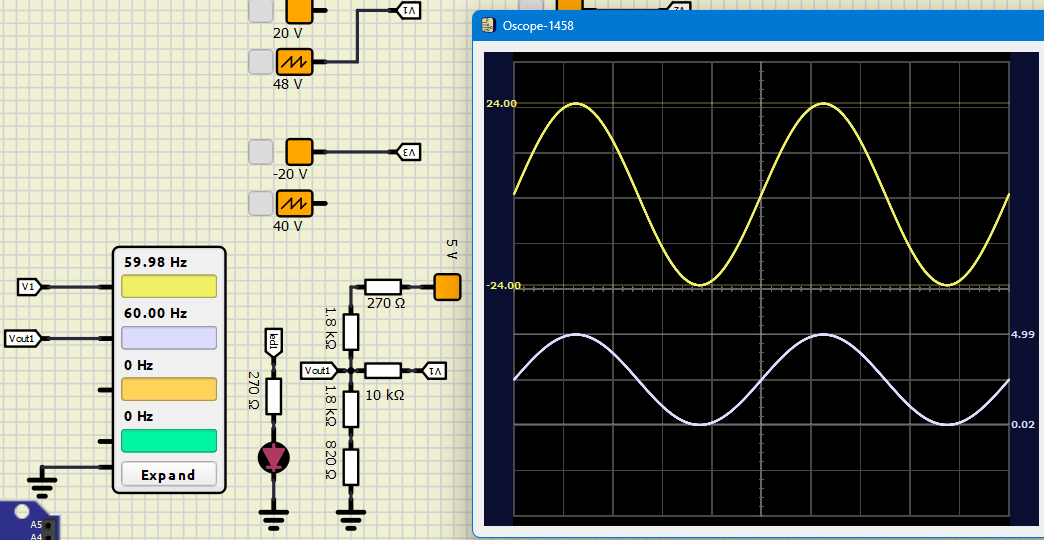
\includegraphics[width=14cm]{Imagenes/volt.png}
    \caption{Verificación del ``convertidor de tensión''. La entrada es la señal senoidal amarilla y la señal violeta es la salida.}
    \label{volt-convert}
\end{figure}

\subsection{Switch AC/DC}
Se implementó un switch que pueda escoger entre tomar datos en corriente directa (DC) o en tomar datos en corriente alterna (AC). Nota: se utiliza la resistencia de pull-up interna que tiene el pin \cite{pullup}.

\subsubsection{Prueba en DC}

Para realizar la prueba en DC, se decidió conectar una fuente distinta de tensión en cada uno de los canales, de manera que a un circuito se le conecta a una fuente de 20V, al segundo una de 23V, al tercero -20V y al ultimo una de -22V. Esto se realiza con el fin de probar distintos casos y poder observar qué sucede cuando el Arduino UNO detecta una tensión mayor a 20V o menor a -20V, tal y como se muestran en la figura \ref{FuncaionamientoDC}.

\begin{figure}[H]
    \centering
    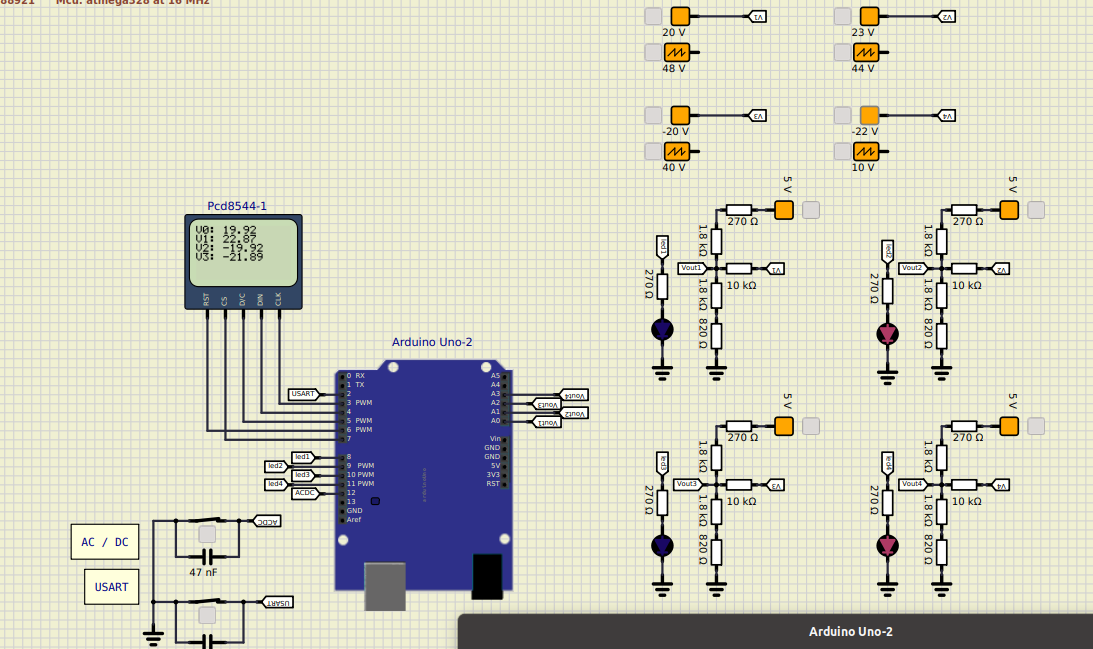
\includegraphics[width=\textwidth]{Imagenes/Funcionamiento_DC.png}
    \caption{Circuito en pruebas en DC.}
    \label{FuncaionamientoDC}
\end{figure}

\begin{figure}[H]
    \centering
    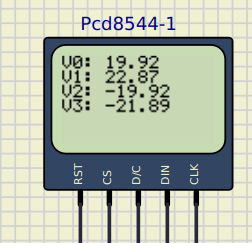
\includegraphics[width=0.6\textwidth]{Imagenes/Valores_pantallaLCD.png}
    \caption{Valores en pantalla LCD en pruebas en DC.}
    \label{PantallaLCD}
\end{figure}

Como se observa en la figura \ref{PantallaLCD}, el valor de V1 sobrepasa los 20 volts, y el valor de V3 es menor a los -20V, entonces los diodos LED de ambos circuitos se encienden como se observa en la figura \ref{FuncaionamientoDC}.

\subsubsection{Prueba en AC}
Para este caso, se cambia de posición el switch para medir en AC y mostrar las tensiones en RMS. Ahora, al igual que en las pruebas de DC, se colocan 4 generadores de señales, cada uno con una amplitud distinta, de manera que el primer circuito reciba un tensión entre [-24, 24] V, el segundo circuito reciba un tensión entre [-22, 22] V, el tercer circuito reciba un tensión entre [-20, 20] Vy el ultimo circuito una tensión entre [-5, 5] V, tal y como se muestra en la figura \ref{FuncaionamientoAC}.

\begin{figure}[H]
    \centering
    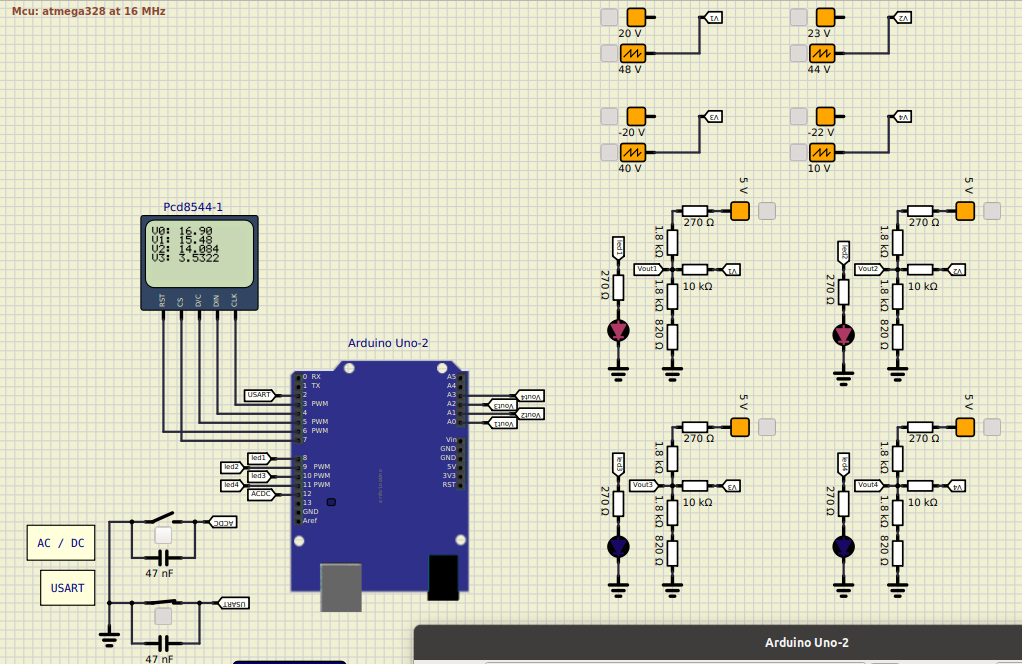
\includegraphics[width=\textwidth]{Imagenes/Funcionamiento_AC.png}
    \caption{Circuito en pruebas en AC.}
    \label{FuncaionamientoAC}
\end{figure}

\begin{figure}[H]
    \centering
    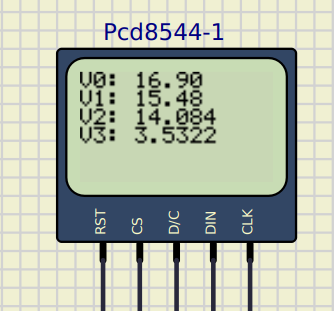
\includegraphics[width=0.6\textwidth]{Imagenes/Valores_pantallaLCD_AC.png}
    \caption{Valores en pantalla LCD en pruebas en DC.}
    \label{PantallaLCD_AC}
\end{figure}

Los valores que muestra la pantalla LCD, son valores RMS, esto quiere decir que se toma el valor de tensión y se divide por raíz de 2, entonces tomando como ejemplo la primera medición se tiene que
\begin{equation}
    V_{rms} = \frac{24}{\sqrt{2}} = 16.97V.
\end{equation}

Como se observa en la ecuación anterior, el valor no es exacto al compararlo con el voltímetro, ciertos decimales cambian, la razón de esto es que cuando se realizó el diseño de las resistencias, se tuvieron que adaptar o poner los valores mas cercanos a los valores comerciales, por ende da como resultado un pequeño cambio en los decimales, pero esta diferencia es muy pequeña y no genera mayor problema. En los circuitos que el arduino detecta un valore de tensión mayor a los 20 V, los cuales serian los primeros 2 circuitos, el diodo LED de alarma se enciende, dando a señalar que se sobrepaso dicho valor de tensión.

\subsection{Switch Serial}
Se implementó un switch que habilita la comunicación serial con otra computadora de manera que envía datos de forma serial, como se observan el las figuras \ref{SerialDC} y \ref{SerialAC}. Nota: se utiliza la resistencia de pull-up interna que tiene el pin \cite{pullup}.

\subsubsection{Prueba en DC}
Para las pruebas en DC, al igual que en las pruebas del switch AD/DC, se conectan 4 diferentes fuentes de tensión para simular los valores en DC, y se abre la comunicación UART, como se observa en la figura \ref{monitor_DC}.

\begin{figure}[H]
    \centering
    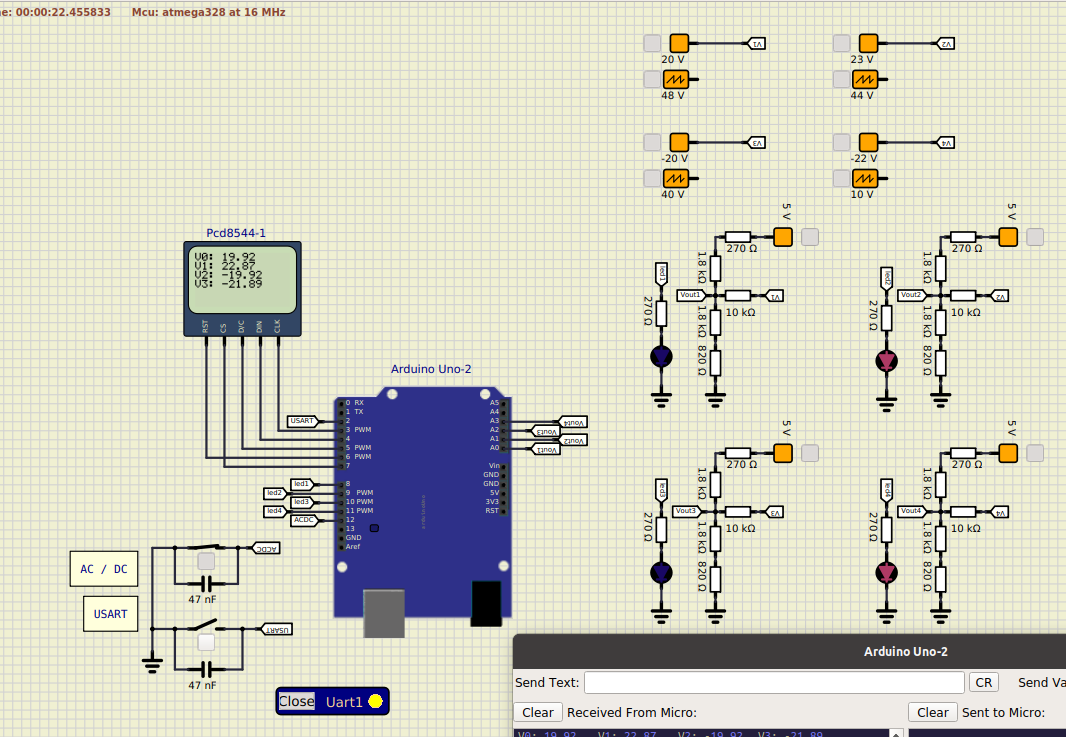
\includegraphics[width=\textwidth]{Imagenes/Circuit_Comu_DC.png}
    \caption{Circuito en pruebas de comunicación serial en DC.}
    \label{SerialDC}
\end{figure}

\begin{figure}[H]
    \centering
    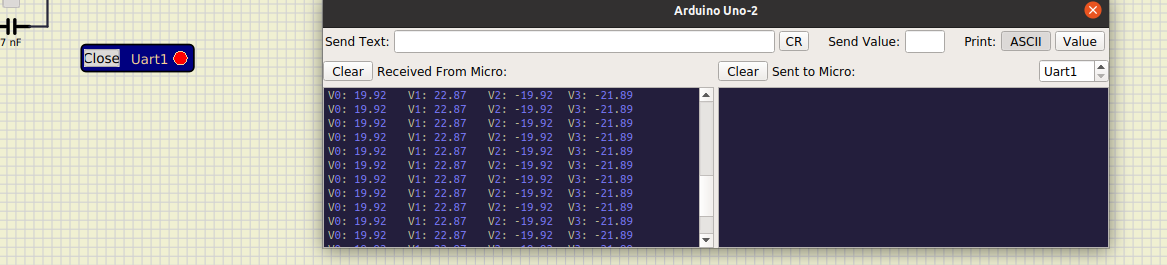
\includegraphics[width=\textwidth]{Imagenes/Comunicacion_Seria_DC.png}
    \caption{Monitor de comunicación Serial en DC y bloque UART.}
    \label{monitor_DC}
\end{figure}

Se puede observar de la figura \ref{monitor_DC}, que el bloque UART esta activado, y que el monitor seria esta recibiendo los datos que se obtiene al hacer la medición en DC, estos datos se envían con un cierto retraso.

\subsubsection{Prueba en AC}

Para las pruebas en AC, al igual que en las pruebas del switch AD/DC, se conectan 4 diferentes generadores de tensión para simular los valores en AC, [-24, 24] V, [-22, 22] V, [-20, 20] V, [-5, 5] V y se abre la comunicación UART, como se observa en la figura \ref{monitor_AC} de manera que permita enviar datos.

\begin{figure}[H]
    \centering
    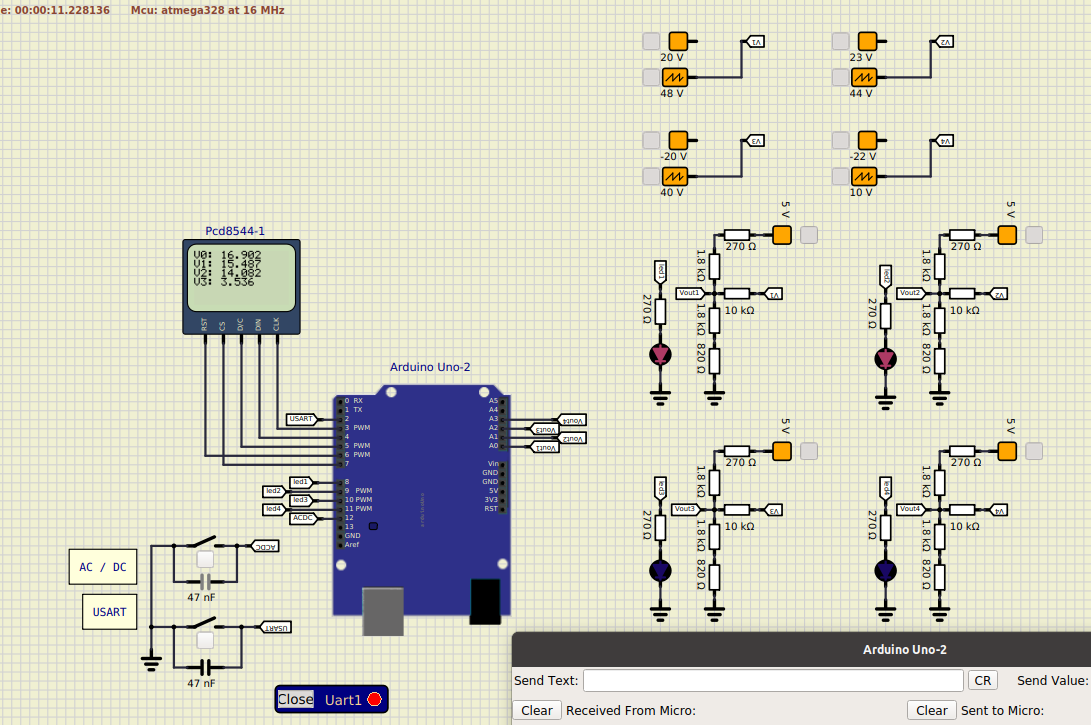
\includegraphics[width=\textwidth]{Imagenes/Circuit_Comu_AC.png}
    \caption{Circuito en pruebas de comunicación serial en AC.}
    \label{SerialAC}
\end{figure}

\begin{figure}[H]
    \centering
    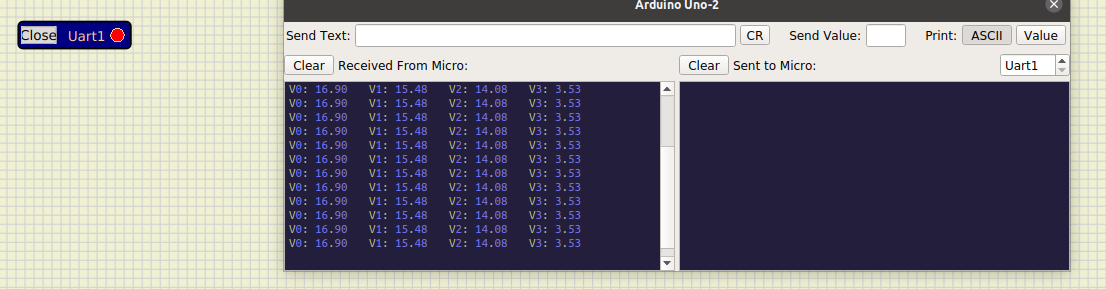
\includegraphics[width=\textwidth]{Imagenes/Comunicacion_Seria_AC.png}
    \caption{Monitor de comunicación Serial en ACy bloque UART.}
    \label{monitor_AC}
\end{figure}

Como se observa en la figura \ref{monitor_AC}, se observa que se esta dando correctamente el envió de datos, permitiendo que otra computadora reciba correctamente los datos, y estos datos se envían de forma serian, ya que primero se envía los datos de V0, V1, V2 y V3, luego se espera un retraso y vuelve tomar medidas y los vuelve a enviar, de manera que toma medidas constantemente y los envía a la otra computadora.

\subsection{Script de Python}
Las figuras \ref{dc1}, \ref{dc2}, \ref{ac1} y \ref{ac2} ilustran que las lecturas son mostrados en la terminal y en el archivo \tt{csv}. Por lo tanto, se concluye que el script funciona para capturar las lecturas por medio de comunicación serial y guardarlas en un archivo csv.
\begin{figure}
    \centering
    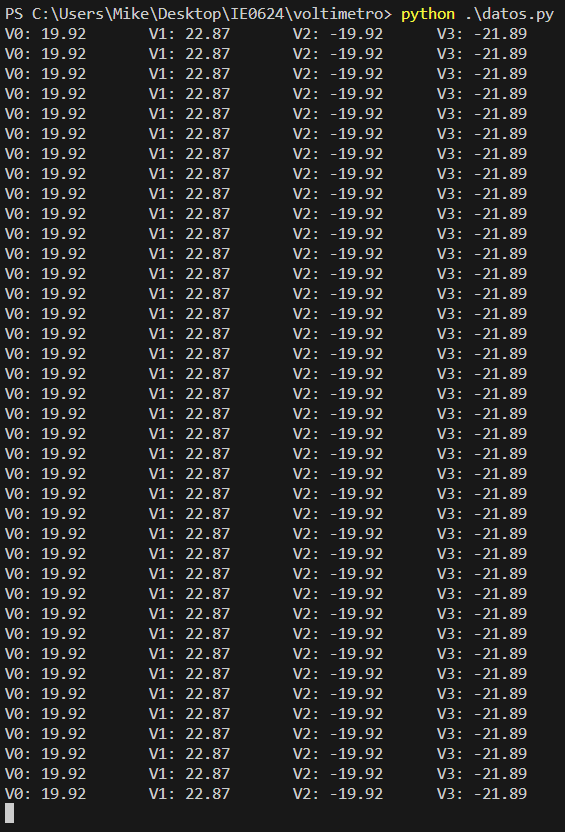
\includegraphics[width=10cm]{Imagenes/DC-save.png}
    \caption{Lecturas de las tensiones DC siendo mostrados en la terminal de la PC.}
    \label{dc1}
\end{figure}

\begin{figure}
    \centering
    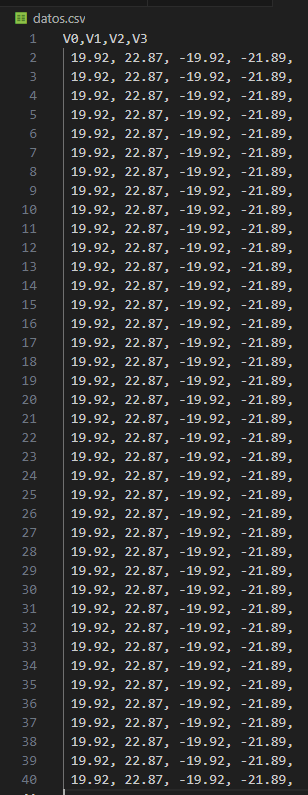
\includegraphics[width=6cm]{Imagenes/DC-saved.png}
    \caption{Lecturas de las tensiones en DC guardadas en el archivo \tt{csv}.}
    \label{dc2}
\end{figure}

\begin{figure}
    \centering
    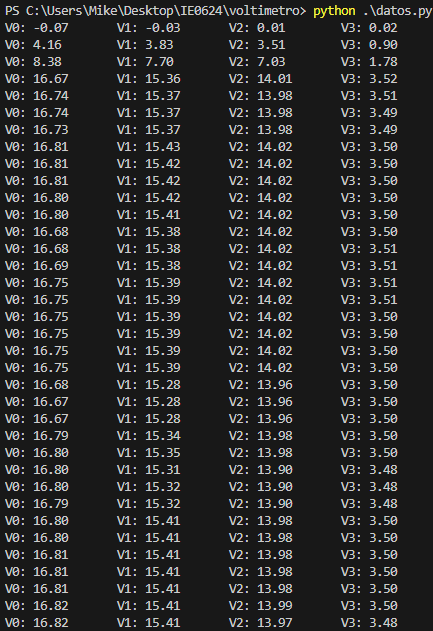
\includegraphics[width=10cm]{Imagenes/AC-save.png}
    \caption{Lecturas de las tensiones AC siendo mostrados en la terminal de la PC.}
    \label{ac1}
\end{figure}

\begin{figure}
    \centering
    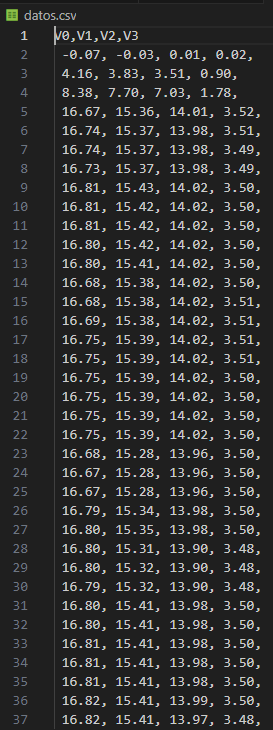
\includegraphics[width=6cm]{Imagenes/AC-saved.png}
    \caption{Lecturas de las tensiones en AC guardadas en el archivo \tt{csv}.}
    \label{ac2}
\end{figure}


































